\documentclass[12pt]{article}
\usepackage{graphicx}
\usepackage{float}
\begin{document}
\tableofcontents
% https://github.com/anadallora/SNAC/blob/master/protocol%20v4.pdf
\section{Introduction}
Dementia has been identified as one of the fastest growing difficulties facing the world. A recent report suggests that in 2015 there were 46 million people with a diagnosis of dementia and that number is expected to hit 131.5 million by 2050 \cite{Prince2015}. The report also states that the worldwide cost of dementia in 2018 is estimated to be in the region of one trillion US dollars.
\par
In 2009, the Department of Health designed it's National Dementia strategy and as part of this made early diagnosis and support one of it's key priorities \cite{England2009}. A lot of work has gone into trying to find ways of improving the early diagnosis of Alzheimer's Disease (AD) and Mild Cognitive Impairment (MCI) with research focused on two areas - identifying biological markers and analyzing the cognitive decline of those who are suspected to have the disease \cite{Taler2008}. As described above, the numbers of those suffering from AD and MCI are going to increase as the population ages \cite{Prince2015} and thus it is important that we utilize technology wherever possible to aid clinicians in the detection of MCI and AD. At the present time diagnosis is typically conducted at memory clinics by trained clinicians \cite{Boschi2017}. I theorize that we may be able to enable an earlier diagnosis of those with MCI and AD using samples of spontaneous speech, natural language processing (NLP) and machine learning (ML).
\par
There is a large body of research that looks at the decline in language in those with MCI and AD \cite{Taler2008, Boschi2017}. However there is conflicting evidence in these studies about which declining language factors are associated of MCI and AD \cite{Taler2008, Boschi2017}. Research therefore should look at these features in more detail and a clarification of this currently disorganised picture should go some way to helping researchers further understand the disease and it's progression. Another area of focus for research of this nature is the process of collecting appropriate language samples. Whilst collecting samples of language is comparatively unintrusive, researchers recognise that these samples require a rich sample of language that potentially cannot be generated by tasks such as the picture description task. Therefore, it would be useful to explore whether spontaneous discourse such a semi-structured interview, has the ability to put pressure on both the cognitive and linguistic systems in the same way as traditional cognitive tests such that it might be able to distinguish between healthy controls, those with MCI and those with AD. There is some evidence to support this. Berisha et al \cite{Berisha2015}, has shown through a longitudinal language analysis of spontaneous speech that there are marked differences in this process between those who would go on to have a diagnosis of AD and a healthy control. 
\par
The potential impact of this research in this area is immense. Research has shown that early diagnosis of people with AD or MCI improves sufferers quality of life and can, in some cases, slow the progress of the disease. Early diagnosis can increase the number of research opportunities for understanding the early stages of dementia and how the disease progresses so that more research can be conducted which may, in the future, lead to new treatments and other interventions.

The aim of my research is to find less burdensome ways of detecting dementia without the use of invasive procedures (taking bloods, or using medical equipment such as MRI's and EEG's) and without resorting to to time-consuming and expensive psychological tests. There is a lot of research into the analysis of language as a bio-marker for MCI and Early Dementia. Given that sampling a person's language is relatively effortless, my research looks at whether we can find bio-markers of MCI and Early Dementia in natural language.\newline
Concerns: Language and Memory are quite naturally intertwined and it would be difficult to test one without some reliance on the other. I'm not going to control for memory problems as a potential confound, but does this weaken the research? How do I defend this? \newline
\par 
Introduction to the problem of dementia in the context of the wider world including quality of life and financial implications. Exploration of dementia as a syndrome rather than a disease, and a look at the different variants of dementia. A look at the rationale behind research into the early diagnosis of dementia as well as a brief look at what has been done in the area (wide context, so pharmacological and psychological). \newline

The question to be addressed in this systematic review is how has the field of machine learning and natural language processing addresses language deterioration in the diagnosis of Mild Cognitive Impairment and Early Alzheimer's Disease.
\section{Research Protocol}
\subsection{Research Question}
The main research question this SLR aims to address is: “How has the field of machine learning and natural language processing addresses language deterioration in the diagnosis of Mild Cognitive Impairment and Early Alzheimer's Disease?”. This main question was decomposed further into five research questions:
\begin{enumerate}
	\item RQ1: Which ML and MS techniques are being used in the dementia and comorbidities research?
	\item RQ2: What data characteristics (variables, determinants and indicators) are being considered when applying the ML or/and MS techniques (physiological, demographic/social, genetics, lifestyle etc)?
	\item RQ3: What are the goals of the studies that employ ML or MS techniques for prognosis of dementia and comorbidities?
	\item RQ4: How is data censoring being handled in the studies?
	\item RQ5: Do the studies focus on individuals or populations?
\end{enumerate}
\subsection{Search Process}

To address the research questions, a search string was defined using the PICO approach, which decomposes the main question into four parts: population, intervention, comparison and outcome. The comparison component was discarded because the SLR was mainly concerned with a characterization. For each of the remaining components, keywords were derived and their rationale can be represented as follows:
\begin{enumerate}
	\item Population: Studies that present research on dementia and comorbidities. Dementia’s keywords were selected from the “Systematized Nomenclature of Medicine–Clinical Terms” and selected by A4. Comorbidities’ keywords were extracted from the Marengoni et al. SLR in this topic.
	\item Intervention: ML or MS techniques. The ML keywords were selected from the branch “Machine Learning Approaches” of the “2012 ACM Computing Classification System”. The MS keywords were selected by A2.
	\item Outcome: Prognosis on dementia and comorbidies. The prognosis keywords were provided
by A4.
\end{enumerate}

The automated searches were performed in the Pubmed, Web of Science and Scopus databases. Table 1 shows the search string used for the Pubmed automated search, but note that this search string was adapted to each of the other databases’ search context.

\begin{table}
	\begin{tabular}{ p{12cm} }
	\hline
	(dementia OR MCI OR Mild Cognitive Impairment OR Alzheimer's OR Mild Neurocognitive Disorder OR AD) AND TOPIC: (machine learning OR Data Mining OR Decision Support System OR NLP OR Natural 			Language Processing) AND TOPIC: (prognosis OR prognostic estimate OR predictor OR prediction OR model OR patterns OR diagnosis OR diagnostic OR forecasting OR projection OR Deep Language Model 		OR Deep Neural Network) AND TOPIC: (classification OR regression OR kernel OR support vector machines OR Gaussian Process OR Bayesian Network OR Factor Analysis OR Deep Learning OR Neural 			Networks OR Maximum Likelihood OR Principal Component Analysis OR Markov OR Linear Model OR Mixture Model OR Perceptron Algorithm OR Logical Learning OR relational learning OR Supervised 				Learning OR Unsupervised Learning OR clustering OR Decision Tree) AND TOPIC: (Language OR Cognitive OR Speech OR Conversation OR Connected Speech OR Picture Description OR Discourse Analysis OR 		Verbal Fluency)  \\ \hline
	Searched - 4th April 2019 - Generated 1257 Articles \\
	\hline
	\end{tabular}
	\caption[Table caption text]{Search Terms for Web of Science database}
	\label{table:name}
\end{table}



\begin{table}
	\begin{tabular}{ p{3cm} | p{3cm} | p{3cm} | p{3cm} }
	\hline
	Scopus & Web of Science & PubMed & IEEE Xplore \\ \hline
	1002 & 991 & 376 & 230 \\ 
	\hline
	\end{tabular}
	\caption[Table caption text]{Totals from each database}
	\label{table:name}
\end{table}


\subsection{Primary Study Selection}
Firstly, the results from the automated searches from the three selected sources (Scopus, Pubmed and Web of Science) will have their duplicates removed, and this set of possible primary studies will be assessed by the evaluation of the titles and abstracts according to the defined inclusion and exclusion criteria. The result from this is our first selected subset (Selected Subset 1). The next phase is to look at the reference lists of papers in Selected Subset 2 and identify any papers missed in the automated searches. This is our second selected subset (Selected Subset 2). \par 
Each paper in these subsets will be fully read and assessed for it's quality, using the process documented further down. Any papers that meet the established criteria will be included as a primary study for this systematic review. 

\begin{figure}[H]
\centering
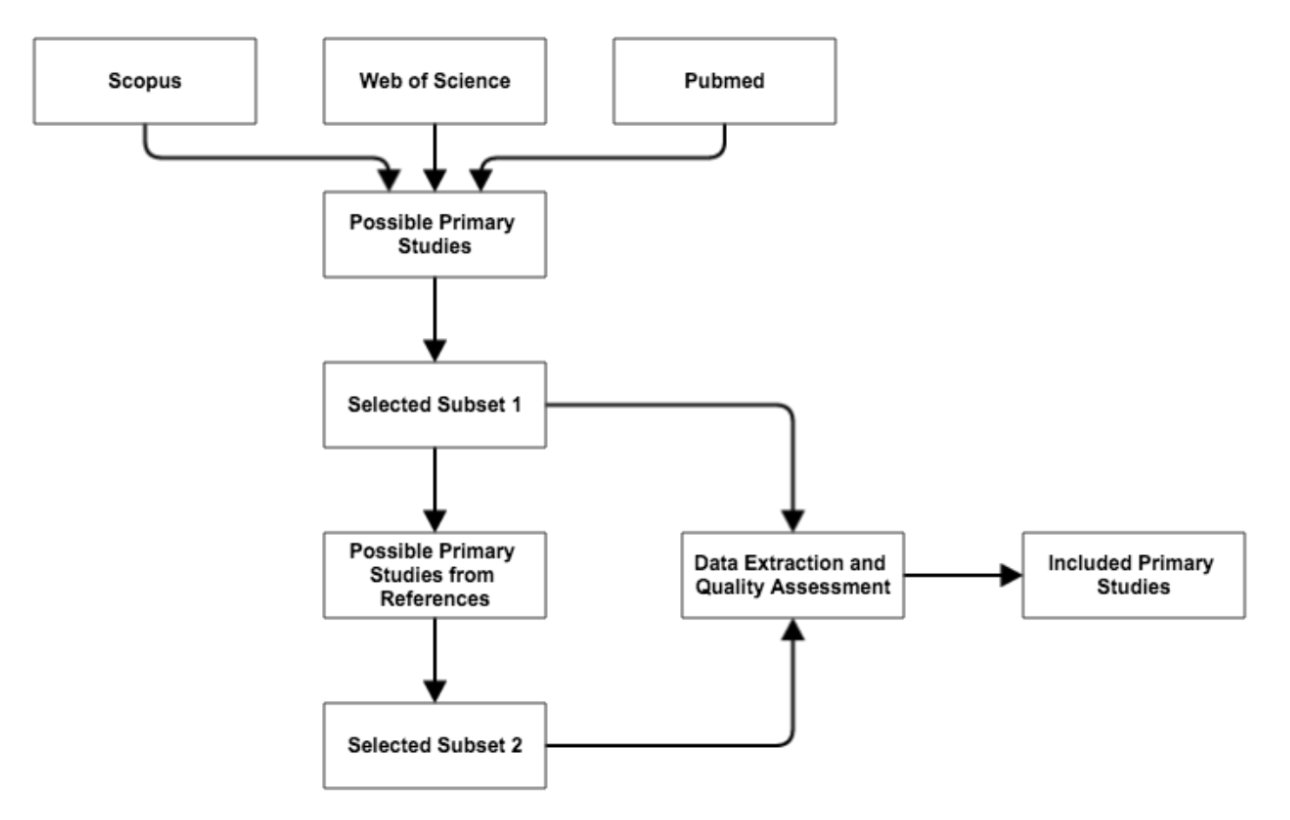
\includegraphics[width=300px, height=150px]{images/PRISMA - Chart.png}
\caption{Selection Chart}
\end{figure}
\subsection{Study Quality Assessment}
The papers selected will be full read and will then pass through an assessment of quality. The assessment will answer the following questions. 
\begin{table}
	\begin{tabular}{ p{6cm} | p{6cm} }
	\hline
	Question & Rating Scale \\ \hline
	Are the aims of the study clearly stated? & Yes=1; Partly=0.5; No=0 \\ \hline
	Does the study describe clearly the population being studied? & Yes=1; Partly=0.5; No=0 \\ \hline
	Was the sample size justified? & Yes=1; Partly=0.5; No=0 \\ \hline
	Is the sample representative of the population to which the results will generalize? & Yes=1; Partly=0.5; No=0 \\ \hline
	Were the limitations of the study reported either during the explanation of the study design or during the discussion of the study results? & Yes=1; Partly=0.5; No=0 \\ \hline
	Were the findings clearly reported? & Yes=1; Partly=0.5; No=0 \\ \hline
	\hline
	Are the measures used in the study clearly defined? & Yes=1; Partly=0.5; No=0 \\ \hline
	Are the measuses used in the study valid? & Yes=1; Partly=0.5; No=0 \\ \hline
	Are the measures used in the study clearly described? & Yes=1; Partly=0.5; No=0 \\ \hline
	\hline
	Is/are the technique(s) being employed clearly described? & Yes=1; Partly=0.5; No=0 \\ \hline
	In the case of more than one technique, was the statistical significance assessed? & Yes=1; Partly=0.5; No=0 \\ \hline
	Was a senstivity analysis carried out to assess if the results were due to certain inputs? & Yes=1; Partly=0.5; No=0 \\ \hline
	\end{tabular}
	\caption[Table caption text]{Paper quality assessment}
	\label{table:name}
\end{table}




\subsection{Data Extraction}
\subsection{Data Synthesis and Reporting}

\appendix
\section{\\Appendix A - Change Log}

\section{\\Appendix B - Searches}
\begin{table}
	\begin{tabular}{ p{12cm} }
	\hline
	(dementia OR MCI OR Mild Cognitive Impairment OR Alzheimer's OR Mild Neurocognitive Disorder OR AD) AND TOPIC: (machine learning OR Data Mining OR Decision Support System OR NLP OR Natural 			Language Processing) AND TOPIC: (prognosis OR prognostic estimate OR predictor OR prediction OR model OR patterns OR diagnosis OR diagnostic OR forecasting OR projection OR Deep Language Model 		OR Deep Neural Network) AND TOPIC: (classification OR regression OR kernel OR support vector machines OR Gaussian Process OR Bayesian Network OR Factor Analysis OR Deep Learning OR Neural 			Networks OR Maximum Likelihood OR Principal Component Analysis OR Markov OR Linear Model OR Mixture Model OR Perceptron Algorithm OR Logical Learning OR relational learning OR Supervised 				Learning OR Unsupervised Learning OR clustering OR Decision Tree) AND TOPIC: (Language OR Cognitive OR Speech OR Conversation OR Connected Speech OR Picture Description OR Discourse Analysis OR 		Verbal Fluency)  \\ \hline
	Searched - 4th April 2019 - Generated 1257 Articles \\
	\hline
	\end{tabular}
	\caption[Table caption text]{Search Terms for Scopus database}
	\label{table:name}
\end{table}

\begin{table}
	\begin{tabular}{ p{12cm} }
	\hline
	(dementia OR MCI OR Mild Cognitive Impairment OR Alzheimer's OR Mild Neurocognitive Disorder OR AD) AND TOPIC: (machine learning OR Data Mining OR Decision Support System OR NLP OR Natural 			Language Processing) AND TOPIC: (prognosis OR prognostic estimate OR predictor OR prediction OR model OR patterns OR diagnosis OR diagnostic OR forecasting OR projection OR Deep Language Model 		OR Deep Neural Network) AND TOPIC: (classification OR regression OR kernel OR support vector machines OR Gaussian Process OR Bayesian Network OR Factor Analysis OR Deep Learning OR Neural 			Networks OR Maximum Likelihood OR Principal Component Analysis OR Markov OR Linear Model OR Mixture Model OR Perceptron Algorithm OR Logical Learning OR relational learning OR Supervised 				Learning OR Unsupervised Learning OR clustering OR Decision Tree) AND TOPIC: (Language OR Cognitive OR Speech OR Conversation OR Connected Speech OR Picture Description OR Discourse Analysis OR 		Verbal Fluency)  \\ \hline
	Searched - 4th April 2019 - Generated 1257 Articles \\
	\hline
	\end{tabular}
	\caption[Table caption text]{Search Terms for ProQuest database}
	\label{table:name}
\end{table}

\begin{table}
	\begin{tabular}{ p{12cm} }
	\hline
	(dementia OR MCI OR Mild Cognitive Impairment OR Alzheimer's OR Mild Neurocognitive Disorder OR AD) AND TOPIC: (machine learning OR Data Mining OR Decision Support System OR NLP OR Natural 			Language Processing) AND TOPIC: (prognosis OR prognostic estimate OR predictor OR prediction OR model OR patterns OR diagnosis OR diagnostic OR forecasting OR projection OR Deep Language Model 		OR Deep Neural Network) AND TOPIC: (classification OR regression OR kernel OR support vector machines OR Gaussian Process OR Bayesian Network OR Factor Analysis OR Deep Learning OR Neural 			Networks OR Maximum Likelihood OR Principal Component Analysis OR Markov OR Linear Model OR Mixture Model OR Perceptron Algorithm OR Logical Learning OR relational learning OR Supervised 				Learning OR Unsupervised Learning OR clustering OR Decision Tree) AND TOPIC: (Language OR Cognitive OR Speech OR Conversation OR Connected Speech OR Picture Description OR Discourse Analysis OR 		Verbal Fluency)  \\ \hline
	Searched - 4th April 2019 - Generated 1257 Articles \\
	\hline
	\end{tabular}
	\caption[Table caption text]{Search Terms for IEEE Xplore database}
	\label{table:name}
\end{table}
\end{document}